\begin{frame}
    \frametitle{Architecture}
    In this section I'll describe the model and the modifications I've made during second phase.
    \subsection{The Model}
    \begin{itemize}
        \item CNN, no other choice for that kind of task.
        \item Started from a known network for image classification.
        \item Hyper parameters tuning
    \end{itemize}
\end{frame}

\begin{frame}
    \frametitle{Architecture (cont.)}
    \begin{figure}
        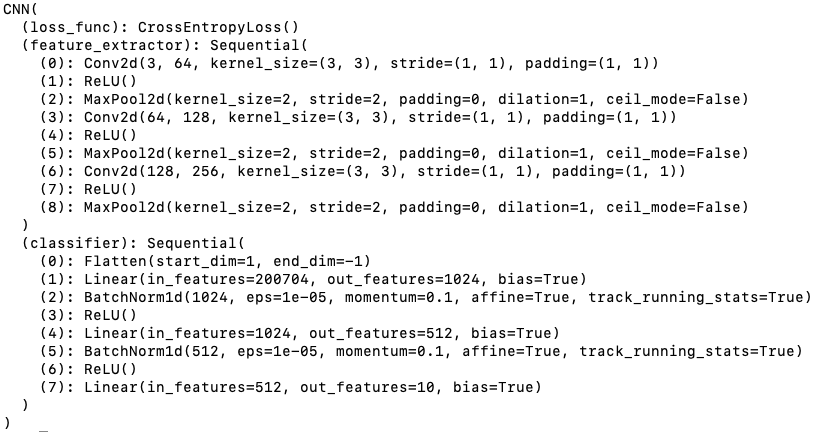
\includegraphics[scale=0.3]{images/architecture}
        \label{fig:architecture}
    \end{figure}

    \begin{figure}

        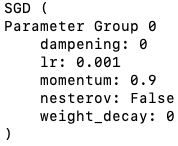
\includegraphics[width=0.15\textwidth]{images/optimizer}
        \label{fig:optimizer}
    \end{figure}
\end{frame}


\begin{frame}
    \frametitle{Architecture - Training}
    \subsection{Training}
    In training phase we train two models, in three steps as followed:
    \begin{enumerate}
        \item<1-> \label{NI} Natural Image:
        \begin{itemize}
            \item A Pre-Trained Resnet18 Model that detects human beings (alongside other)
            \item Fine tune model's top layers with training data
            \item Isn't being used for final classification
            \item Used for Human Model Retraining
        \end{itemize}
        \item<2-> Human Model
        \begin{itemize}
            \item Fine tune Natural Image model's top layer
            \item Add three classes (with\_mask, without\_mask, mask\_weared\_incorrect)
            \item Remove 'person' class in return
            \item Used to determine if the object is a person
        \end{itemize}
        \item<3-> Face Mask Detection
        \begin{itemize}
            \item A model we train from scratch
            \item Used for Human Model Retraining
        \end{itemize}
    \end{enumerate}

    \begin{block}{Implementation Note}<4->
        \begin{itemize}
            \item High RAM and CUDA memory consumption (over 4GB)
            \item Works perfectly on a google-collab machine
            \item Debugged on a pre-trained resnet18
            \item My model is more accurate
            \item Code knows to automatically detect environment and use model accordingly
        \end{itemize}
    \end{block}
\end{frame}

\begin{frame}
    \frametitle{The Testing Pipeline}
    \subsection{Testing Pipeline}
    \begin{itemize}
        \item Take an image
        \item Determine if the object/s in the picture are human (using Human Detection Model model)
        \item Crop the object/s one by one (using first model), \& determine masked/non-masked/partially-masked (using second model)
    \end{itemize}
\end{frame}
